\section{Introduzione}
Con l'identificazione dei modelli vogliamo trovare un modello matematico (una funzione) che leghi, nel miglior modo possibile, un'insieme di dati riguardanti variabili indipendenti con un'insieme di dati dipendenti.

\begin{figure}[htbp]
  \centering
  \[
    \begin{CD}
       @>u>> \framebox{$Y=\Phi(u,\theta)$} @>Y>>
    \end{CD}
  \]
  \caption{Diagramma di un modello statico\label{fig:diagrammamodstat}}
\end{figure}

\begin{itemize}
    \item $Y$ è l'insieme delle variabili dipendenti, ovvero i dati misurati sull'esperimento che vogliamo spiegare con un modello
    \item $u$ è l'insieme delle variabili indipendenti, ovvero dati misurati, o noti a priori, mediante i quali voglio spiegare gli effetti
    \item $\Phi( , )$ è il modello matematico che lega $u$ ad $Y$
    \item $\theta$ parametri incogniti del modello
\end{itemize}

\begin{esempio} % ###########
Per chiarire il concetto di identificazione del modello, prendiamo, ad esempio, una resistenza di cui conosciamo differenza di potenziale $V$ e corrente $I$ e vogliamo trovare il modello che permette di determinare la corrente in funzione della differenza di potenziale.
\begin{figure}[htbp]
  \centering
  \includegraphics[ scale=0.5]{img/resistenza}
  \caption{Schema circuitale di una resistenza\label{fig:resistenza}}
\end{figure}

Dopo alcune misure sperimentali otteniamo:

\begin{figure}[htbp]
  \centering
  \includegraphics[ keepaspectratio]{mathematica/resistenza}
  \caption{In figura è rappresentato l'andamento del modello, confrontato con l'andamento reale del sistema. Presi alcuni campioni si nota l'esistenza di un errore $\varepsilon$ nel modello rispetto alla realtà\label{fig:modelloresistenza}}
\end{figure}

La retta rappresentata nel grafico nella realtà non si verifica mai per via di errori di misura, inoltre, la relazione perfettamente lineare sussiste solo nel caso di una resistenza ideale.
Nel caso di questo esempio la variabile dipendente è la corrente, quindi $Y=I$, mentre la variabile indipendente è la differenza di potenziale, quindi $u=V$; ne consegue che il modello che vogliamo trovare sarà:

  \begin{align*}
    Y&=\Phi (u,\theta) \quad     u=\begin{bmatrix} V_1 \\ V_2 \\ \vdots \\ V_N\end{bmatrix} \quad  Y=\begin{bmatrix} I_1 \\ I_2 \\ \vdots \\ I_N \end{bmatrix}\\
    \theta&=R \vee \theta=\frac{1}{R}
  \end{align*}
  
Per la legge di Ohm sappiamo che la relazione che lega questi due valori è $I=\frac{V}{R}$, quindi il nostro modello sarà:

  \[ \Phi(u,\theta)=u \cdot \theta \vee \Phi(u,\theta)=u \cdot \frac{1}{\theta} \]
  
In questo caso abbiamo un modello lineare nei parametri.
\end{esempio}

\begin{esempio} % ###########
Supponiamo di conoscere la concentrazione plasmotica di un farmaco e che evolve secondo la legge:

  \[ C(t)=a \cdot e^{-\alpha t}+b \cdot e^{-\beta t} \]
  
i cui coefficienti $a$, $b$, $\alpha$, $\beta$ sono da stimare.
Sappiamo che il grafico di $C(t)$ ha un andamento esponenziale inverso, sappiamo, inoltre, che la concentrazione del farmaco è positiva e quindi $C(t)\geq 0$. Effettuano $N$ prelievi nel tempo otteniamo i campioni rappresentati in figura \ref{fig:concfarmaco}:

\begin{figure}[htbp]
  \centering
  \includegraphics[keepaspectratio]{mathematica/andamentofarmaco}
  \caption{Andamento della concentrazione di un farmaco nel sangue. Anche qua vediamo che il modello presenta degli errori rispetto all'andamento reale\label{fig:concfarmaco}}
\end{figure}

In questo caso il modello viene rappresentato in questo modo:

  \begin{align*}
    Y&=\begin{bmatrix} C(t_1)\\C(t_2)\\ \vdots \\ C(t_N) \end{bmatrix}\quad u=\begin{bmatrix} t_1 \\ t_2 \\ \vdots \\t_n \end{bmatrix}=\begin{bmatrix} u_1 \\ u_2 \\ \vdots \\u_n \end{bmatrix} \quad \theta=\begin{bmatrix} a \\ b \\ \alpha \\ \beta \end{bmatrix}=\begin{bmatrix} \theta_1 \\ \theta_2 \\ \theta_3 \\ \theta_4 \end{bmatrix}\\
    C(t_i)&=\theta_1 \cdot e^{-\theta_2 t_i} + \theta_3 \cdot e^{-\theta_4 t_i}
  \end{align*}
  
Da questo ne consegue che il nostro modello sarà:

  \[ \Phi(u,\theta)=\begin{bmatrix} \theta_1 \cdot e^{-\theta_2 t_1} + \theta_3 \cdot e^{-\theta_4 t_1}\\ \vdots  \\ \theta_1 \cdot e^{-\theta_2 t_N} + \theta_3 \cdot e^{-\theta_4 t_N} \end{bmatrix} \]
  
Questo è un esempio di modello non lineare nei parametri, infatti, i parametri $\theta_2$ e $\theta_4$ sono all'esponente, quindi non lineari. Ne consegue che non possiamo scrivere ilmodello come combinazione lineare.
\end{esempio}

\begin{esempio} % ###########
Prendiamo ora come esempio un campione di dati e cerchiamo di approssimare\footnote{mediante interpolazione} l'andamento dei punti con una funzione cubica, come in figura \ref{fig:andamentocubido}.

  \begin{figure}[htbp]
    \centering
    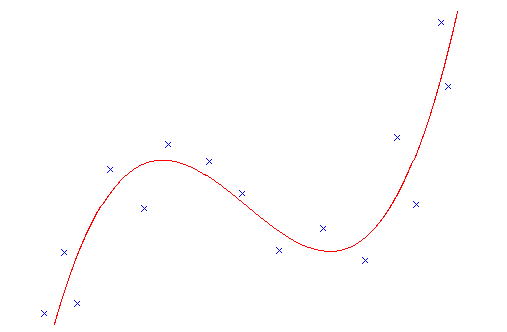
\includegraphics[keepaspectratio]{mathematica/cubica}
    \caption{Funzione cubica per l'interpolazione dei campioni di un processo\label{fig:andamentocubido}}
  \end{figure}

  \[ y=a_0 + a_1x+a_2x^2+a_3x^3 \]
Da qui, gli elementi del nostro modello saranno:

  \[
    Y=\begin{bmatrix} y_1\\y_2\\ \vdots \\ y_N \end{bmatrix}\quad
    u=\begin{bmatrix} x_1 \\ x_2 \\ \vdots \\ x_n \end{bmatrix}=\begin{bmatrix} u_1 \\ u_2 \\ \vdots \\u_n \end{bmatrix}\quad
    \theta=\begin{bmatrix} a_0 \\ a_1 \\ a_2 \\ a_3 \end{bmatrix}=\begin{bmatrix} \theta_1 \\ \theta_2 \\ \theta_3 \\ \theta_4 \end{bmatrix}
  \]
  
e quindi il modello:

  \[ \Phi(u,\theta)=\begin{bmatrix} \theta_1 + \theta_2u_1+\theta_3u_1^2+\theta_4u_1^3  \\ \vdots \\ \theta_1 + \theta_2u_N+\theta_3u_N^2+\theta_4u_N^3 \end{bmatrix} =\begin{bmatrix} 1 \ u_1 & u_1^2 & u_1^3 \\ & \vdots &    \\  1\ u_N & u_N^2 & u_N^3 \end{bmatrix}\cdot \begin{bmatrix} \theta_1 \\ \theta_2 \\ \theta_3 \\ \theta_4 \end{bmatrix} = \Phi(u) \cdot \theta \]
  
L'ultimo passaggio abbiamo potuto farlo perché il modello è lineare nei parametri, altrimenti, come nell'esempio precedente, non avremmo potuto ottenere questa semplificazione. La matrice $\Phi(u)$ che abbiamo ottenuto è detta matrice di sensitività \index{Matrice di sensistività} ed è costituita da tante colonne quanti sono i parametri e tante righe quante le osservazioni disponibili.
\end{esempio}

\begin{esempio} % ###########
Supponiamo di disporre di $q$ variabili e di voler spiegare $Y$ in funzione delle variabili; la prima approssimazione che si può fare è di tipo lineare e dire quindi che $Y$ è generata per combinazione lineare delle variabili di cui disponiamo. Questa forzatura alla linearità della funzione è detta regressione lineare \index{Regressione lineare}. Ovviamente non è detto che questa approssimazione sia esatta o sia la migliore, ma sicuramente è la più semplice da trattare e quindi preferibile quando possibile. La regressione lineare possiamo rappresentarla come combinazione lineare e quindi:

  \[ y(t)=\sum_{i=1}^{N} {\theta_i \cdot u_i(t)} \]
  
Nella rappresentazione come modello:

  \[ Y=\Phi(u,\theta)=\Phi(u) \cdot \theta \]
\end{esempio}

Dopo questa serie di esempi è evidente che il nostro scopo è quello di stimare il vettore dei parametri , dato che sono noti, rispettivamente sono i risultati e le variabili note a priori dal campione.
